\documentclass[8pt,aspectratio=169]{beamer}
\usetheme{Madrid}
\usepackage{graphicx}
\usepackage{booktabs}
\usepackage{adjustbox}
\usepackage{multicol}
\usepackage{amsmath}
\usepackage{listings}
\usepackage{xcolor}

% Color definitions
\definecolor{mlblue}{RGB}{0,102,204}
\definecolor{mlpurple}{RGB}{51,51,178}
\definecolor{mllavender}{RGB}{173,173,224}
\definecolor{mllavender2}{RGB}{193,193,232}
\definecolor{mllavender3}{RGB}{204,204,235}
\definecolor{mllavender4}{RGB}{214,214,239}
\definecolor{mlorange}{RGB}{255, 127, 14}
\definecolor{mlgreen}{RGB}{44, 160, 44}
\definecolor{mlred}{RGB}{214, 39, 40}
\definecolor{mlgray}{RGB}{127, 127, 127}

% Additional colors for template compatibility
\definecolor{lightgray}{RGB}{240, 240, 240}
\definecolor{midgray}{RGB}{180, 180, 180}

% Apply custom colors to Madrid theme
\setbeamercolor{palette primary}{bg=mllavender3,fg=mlpurple}
\setbeamercolor{palette secondary}{bg=mllavender2,fg=mlpurple}
\setbeamercolor{palette tertiary}{bg=mllavender,fg=white}
\setbeamercolor{palette quaternary}{bg=mlpurple,fg=white}

\setbeamercolor{structure}{fg=mlpurple}
\setbeamercolor{section in toc}{fg=mlpurple}
\setbeamercolor{subsection in toc}{fg=mlblue}
\setbeamercolor{title}{fg=mlpurple}
\setbeamercolor{frametitle}{fg=mlpurple,bg=mllavender3}
\setbeamercolor{block title}{bg=mllavender2,fg=mlpurple}
\setbeamercolor{block body}{bg=mllavender4,fg=black}

% Remove navigation symbols
\setbeamertemplate{navigation symbols}{}

% Clean itemize/enumerate
\setbeamertemplate{itemize items}[circle]
\setbeamertemplate{enumerate items}[default]

% Reduce margins for more content space
\setbeamersize{text margin left=5mm,text margin right=5mm}

% Command for bottom annotation (Madrid-style)
\newcommand{\bottomnote}[1]{%
\vfill
\vspace{-2mm}
\textcolor{mllavender2}{\rule{\textwidth}{0.4pt}}
\vspace{1mm}
\footnotesize
\textbf{#1}
}

% Python code listing style
\lstdefinestyle{python}{
    language=Python,
    basicstyle=\ttfamily\tiny,
    keywordstyle=\color{mlblue}\bfseries,
    stringstyle=\color{mlgreen},
    commentstyle=\color{mlgray}\itshape,
    numberstyle=\tiny\color{mlgray},
    numbers=left,
    numbersep=3pt,
    frame=single,
    framerule=0.5pt,
    rulecolor=\color{mllavender2},
    backgroundcolor=\color{mllavender4},
    breaklines=true,
    breakatwhitespace=true,
    tabsize=4,
    showstringspaces=false,
    morekeywords={self, True, False, None}
}

\lstset{style=python}

\title{Blockchain Fundamentals}
\subtitle{Cryptocurrency and Blockchain Technology -- Lesson 1 of 4}
\author{Prof. Dr. Joerg Osterrieder}
\institute{University Lecture Series}
\date{\today}

\begin{document}

% ==================== SLIDE 1: TITLE ====================
\begin{frame}[plain]
\vspace{2cm}
\begin{center}
{\Huge Blockchain Fundamentals}\\[0.5cm]
{\Large Cryptocurrency and Blockchain Technology}\\[0.3cm]
{\normalsize Lesson 1 of 4}\\[2cm]
{\normalsize Prof. Dr. Joerg Osterrieder}\\[0.3cm]
{\small \today}
\end{center}
\end{frame}

% ==================== SLIDE 2: OUTLINE ====================
\begin{frame}[t]{Today's Agenda}
\begin{columns}[T]
\column{0.48\textwidth}
\textbf{Part 1: What is Blockchain?}
\begin{itemize}
\item History and origins
\item Definition and key properties
\item Real-world applications
\end{itemize}

\vspace{0.5em}
\textbf{Part 2: Block Structure}
\begin{itemize}
\item Anatomy of a block
\item Block header and body
\item Merkle trees
\item How blocks link together
\end{itemize}

\column{0.48\textwidth}
\textbf{Part 3: Consensus Mechanisms}
\begin{itemize}
\item The double-spending problem
\item Proof of Work (PoW)
\item Proof of Stake (PoS)
\end{itemize}

\vspace{0.5em}
\textbf{Part 4: Python Implementation}
\begin{itemize}
\item Building a simple blockchain
\item Mining demonstration
\item Chain validation
\end{itemize}
\end{columns}

\bottomnote{Duration: 45 minutes | This lesson provides the foundational concepts for understanding blockchain technology.}
\end{frame}

% ==================== SECTION 1: WHAT IS BLOCKCHAIN? ====================
\section{What is Blockchain?}

\begin{frame}[t]
\vfill
\centering
\begin{beamercolorbox}[sep=8pt,center]{title}
\usebeamerfont{title}\Large Section 1: What is Blockchain?\par
\end{beamercolorbox}
\vfill
\end{frame}

% ==================== SLIDE 3: HISTORY ====================
\begin{frame}[t]{The Birth of Blockchain}
\begin{columns}[T]
\column{0.48\textwidth}
\textbf{October 31, 2008}

Satoshi Nakamoto publishes the Bitcoin whitepaper:

\vspace{0.5em}
\begin{center}
\textit{``Bitcoin: A Peer-to-Peer Electronic Cash System''}
\end{center}

\vspace{0.5em}
\textbf{Key Innovation:}
\begin{itemize}
\item First practical solution to the \textcolor{mlred}{double-spending problem}
\item No trusted third party required
\item Completely decentralized
\end{itemize}

\column{0.48\textwidth}
\textbf{Timeline}
\begin{itemize}
\item \textbf{2008:} Whitepaper published
\item \textbf{Jan 3, 2009:} Genesis block mined
\item \textbf{2009:} First Bitcoin transaction
\item \textbf{2010:} First real-world purchase (10,000 BTC for pizza)
\item \textbf{2015:} Ethereum launches
\item \textbf{2020s:} Institutional adoption
\end{itemize}

\vspace{0.5em}
\textbf{Mystery:} Satoshi's identity remains unknown
\end{columns}

\bottomnote{The 2008 financial crisis provided context for a trustless, decentralized monetary system.}
\end{frame}

% ==================== SLIDE 4: DEFINITION ====================
\begin{frame}[t]{What is a Blockchain?}
\begin{columns}[T]
\column{0.55\textwidth}
\textbf{Definition}

A blockchain is a \textcolor{mlpurple}{\textbf{distributed, immutable ledger}} that records transactions across a network of computers.

\vspace{1em}
\textbf{Breaking it down:}
\begin{itemize}
\item \textbf{Distributed:} Copies exist on many computers (nodes)
\item \textbf{Immutable:} Once written, data cannot be changed
\item \textbf{Ledger:} A record of transactions
\item \textbf{Linked blocks:} Data organized in sequential blocks
\end{itemize}

\vspace{0.5em}
\textbf{Simple analogy:}

Think of it as a \textcolor{mlblue}{shared Google Doc} that:
\begin{itemize}
\item Everyone can read
\item No one can edit past entries
\item New entries require group approval
\end{itemize}

\column{0.42\textwidth}
\textbf{Traditional Database vs Blockchain}

\vspace{0.5em}
\begin{tabular}{p{2cm}|p{2.5cm}}
\toprule
\textbf{Database} & \textbf{Blockchain} \\
\midrule
Centralized & Distributed \\
Admin controls & Network controls \\
Can be edited & Append-only \\
Trust required & Trustless \\
Fast writes & Slower writes \\
\bottomrule
\end{tabular}
\end{columns}

\bottomnote{A blockchain replaces trust in institutions with trust in mathematics and code.}
\end{frame}

% ==================== SLIDE 5: KEY PROPERTIES ====================
\begin{frame}[t]{Key Properties of Blockchain}
\begin{columns}[T]
\column{0.31\textwidth}
\textbf{\textcolor{mlblue}{Decentralization}}

\vspace{0.5em}
No single point of control:
\begin{itemize}
\item No central authority
\item Peer-to-peer network
\item Democratic governance
\item Resistant to shutdown
\end{itemize}

\vspace{0.5em}
\textit{``The network is the authority''}

\column{0.31\textwidth}
\textbf{\textcolor{mlgreen}{Transparency}}

\vspace{0.5em}
Open and verifiable:
\begin{itemize}
\item All transactions public
\item Anyone can audit
\item Real-time verification
\item Pseudonymous (not anonymous)
\end{itemize}

\vspace{0.5em}
\textit{``Trust through verification''}

\column{0.31\textwidth}
\textbf{\textcolor{mlorange}{Immutability}}

\vspace{0.5em}
Permanent record:
\begin{itemize}
\item Data cannot be altered
\item Cryptographic linking
\item Tamper-evident
\item Historical integrity
\end{itemize}

\vspace{0.5em}
\textit{``Written in stone''}
\end{columns}

\vspace{1em}
\begin{center}
\textbf{Together, these properties enable:} \textcolor{mlpurple}{Trustless transactions between strangers}
\end{center}

\bottomnote{These three properties are interdependent -- removing one weakens the others.}
\end{frame}

% ==================== SLIDE 6: APPLICATIONS ====================
\begin{frame}[t]{Real-World Applications}
\begin{columns}[T]
\column{0.48\textwidth}
\textbf{\textcolor{mlblue}{Finance \& Payments}}
\begin{itemize}
\item Cross-border remittances
\item Micropayments
\item Decentralized finance (DeFi)
\item Central bank digital currencies (CBDCs)
\end{itemize}

\vspace{0.5em}
\textbf{\textcolor{mlgreen}{Supply Chain}}
\begin{itemize}
\item Product traceability
\item Authenticity verification
\item Quality assurance
\item Logistics optimization
\end{itemize}

\column{0.48\textwidth}
\textbf{\textcolor{mlorange}{Identity \& Voting}}
\begin{itemize}
\item Self-sovereign identity
\item Secure voting systems
\item Credential verification
\item Privacy-preserving authentication
\end{itemize}

\vspace{0.5em}
\textbf{\textcolor{mlpurple}{Other Applications}}
\begin{itemize}
\item Healthcare records
\item Intellectual property
\item Real estate titles
\item Gaming and NFTs
\end{itemize}
\end{columns}

\vspace{0.5em}
\begin{center}
\fbox{\parbox{0.8\textwidth}{\centering
\textbf{Common thread:} Applications where \textit{trust}, \textit{transparency}, and \textit{immutability} are critical}}
\end{center}

\bottomnote{Not everything needs a blockchain -- it's most valuable where trust is expensive or impossible.}
\end{frame}

% ==================== SLIDE 7: WHY BLOCKCHAIN FOR FINANCE ====================
\begin{frame}[t]{Why Blockchain Matters for Finance}
\begin{columns}[T]
\column{0.48\textwidth}
\textbf{Current Financial System Pain Points}
\begin{itemize}
\item[\textcolor{mlred}{$\times$}] Cross-border payments take 2-5 days
\item[\textcolor{mlred}{$\times$}] High transaction fees (3-7\%)
\item[\textcolor{mlred}{$\times$}] Settlement requires intermediaries
\item[\textcolor{mlred}{$\times$}] Limited access for unbanked
\item[\textcolor{mlred}{$\times$}] Lack of transparency
\item[\textcolor{mlred}{$\times$}] Counterparty risk
\end{itemize}

\column{0.48\textwidth}
\textbf{Blockchain Solutions}
\begin{itemize}
\item[\textcolor{mlgreen}{$\checkmark$}] Near-instant settlement
\item[\textcolor{mlgreen}{$\checkmark$}] Minimal transaction costs
\item[\textcolor{mlgreen}{$\checkmark$}] Direct peer-to-peer transfers
\item[\textcolor{mlgreen}{$\checkmark$}] Financial inclusion
\item[\textcolor{mlgreen}{$\checkmark$}] Full auditability
\item[\textcolor{mlgreen}{$\checkmark$}] Trustless execution
\end{itemize}
\end{columns}

\vspace{1em}
\textbf{Key Financial Innovations:}
\begin{itemize}
\item \textbf{Smart Contracts:} Self-executing agreements with terms written in code
\item \textbf{Tokenization:} Digital representation of real-world assets
\item \textbf{DeFi:} Decentralized lending, borrowing, and trading
\end{itemize}

\bottomnote{The financial industry stands to gain the most from blockchain's efficiency and transparency.}
\end{frame}

% ==================== SECTION 2: BLOCK STRUCTURE ====================
\section{Block Structure}

\begin{frame}[t]
\vfill
\centering
\begin{beamercolorbox}[sep=8pt,center]{title}
\usebeamerfont{title}\Large Section 2: Block Structure\par
\end{beamercolorbox}
\vfill
\end{frame}

% ==================== SLIDE 8: WHAT IS A BLOCK ====================
\begin{frame}[t]{What is a Block?}
\begin{center}
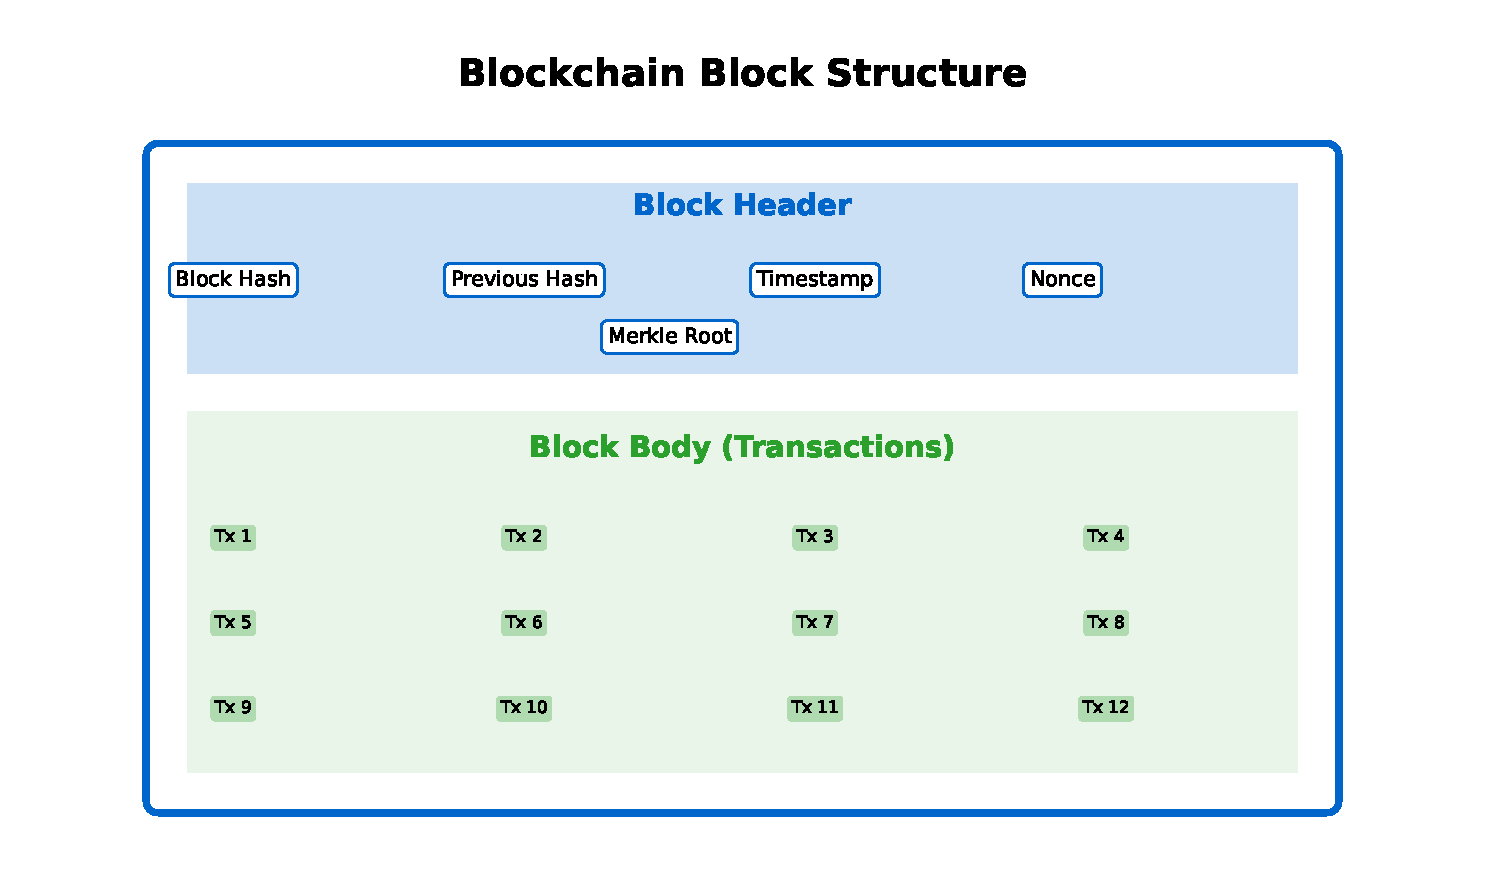
\includegraphics[width=0.85\textwidth]{01_blockchain_structure/01_blockchain_structure.pdf}
\end{center}

\bottomnote{A block is the fundamental unit of a blockchain, containing both metadata (header) and payload (transactions).}
\end{frame}

% ==================== SLIDE 9: BLOCK HEADER ====================
\begin{frame}[t]{Block Header Components}
\begin{columns}[T]
\column{0.48\textwidth}
\textbf{Essential Header Fields}

\vspace{0.5em}
\begin{tabular}{p{2.5cm}p{4cm}}
\toprule
\textbf{Field} & \textbf{Purpose} \\
\midrule
\textcolor{mlpurple}{\textbf{Block Hash}} & Unique identifier for this block \\
\textcolor{mlblue}{\textbf{Previous Hash}} & Links to parent block \\
\textcolor{mlgreen}{\textbf{Timestamp}} & When block was created \\
\textcolor{mlorange}{\textbf{Nonce}} & Mining solution number \\
\textcolor{mlred}{\textbf{Merkle Root}} & Hash of all transactions \\
\bottomrule
\end{tabular}

\vspace{1em}
\textbf{Additional fields (Bitcoin):}
\begin{itemize}
\item Version number
\item Difficulty target
\item Block height (position in chain)
\end{itemize}

\column{0.48\textwidth}
\textbf{How the Hash is Calculated}

\vspace{0.5em}
$$\text{Hash} = \text{SHA256}(\text{Header})$$

\vspace{0.5em}
The hash depends on:
\begin{enumerate}
\item Previous block's hash
\item Merkle root of transactions
\item Timestamp
\item Nonce value
\end{enumerate}

\vspace{0.5em}
\textbf{Key insight:}

Changing \textit{any} field changes the hash completely (avalanche effect)

\vspace{0.5em}
\textbf{Example hash:}
\begin{center}
\tiny\texttt{0000000000000000000a4b...}
\end{center}
\end{columns}

\bottomnote{The block hash is not stored in the block itself -- it's computed from the header data.}
\end{frame}

% ==================== SLIDE 10: MERKLE ROOT ====================
\begin{frame}[t]{Merkle Tree: Efficient Transaction Verification}
\begin{center}
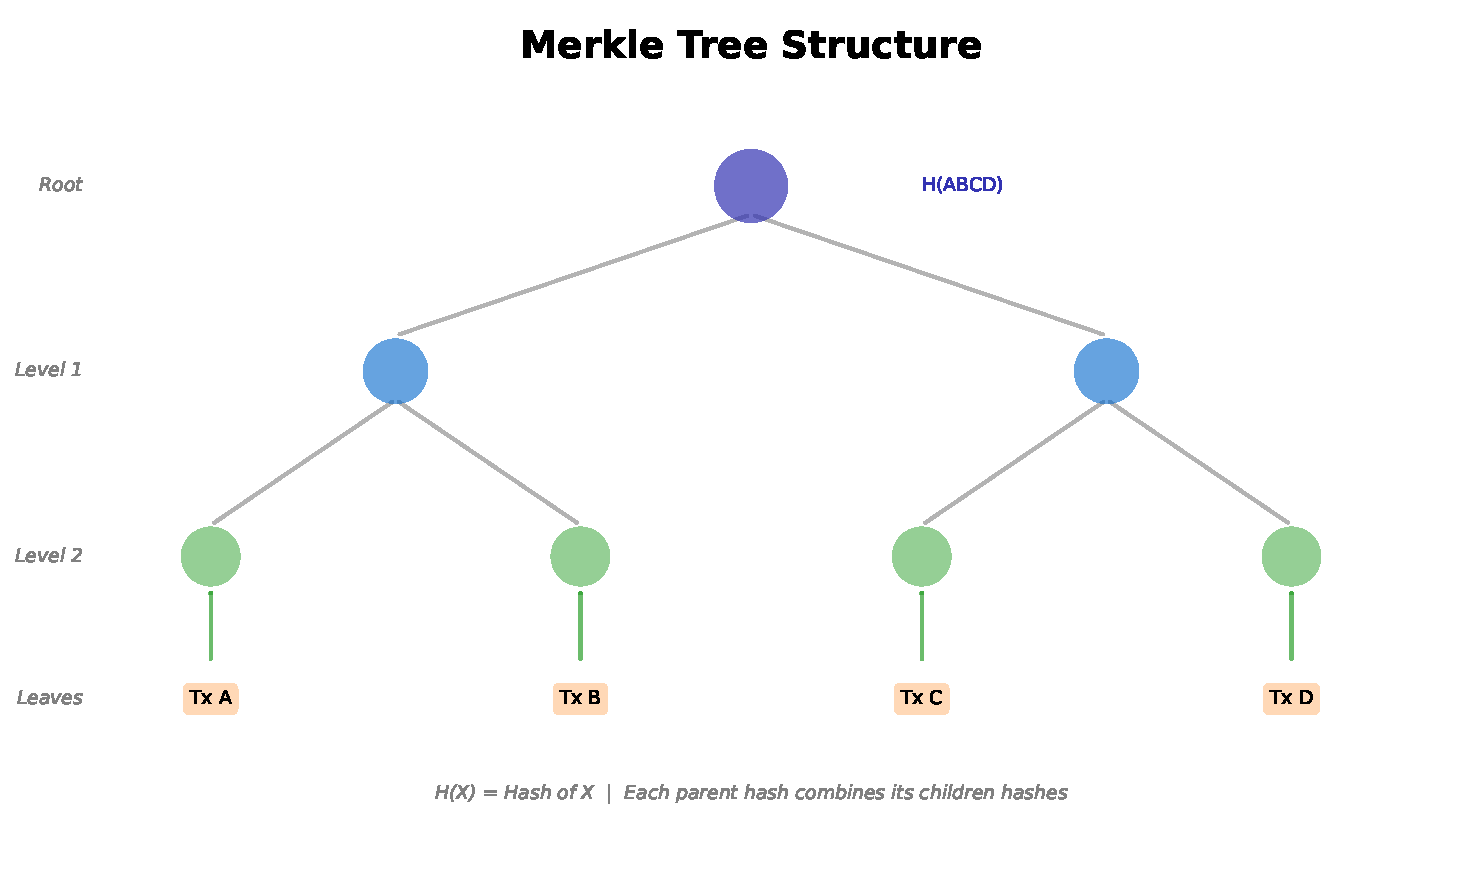
\includegraphics[width=0.75\textwidth]{03_merkle_tree/03_merkle_tree.pdf}
\end{center}

\vspace{0.5em}
\begin{columns}[T]
\column{0.48\textwidth}
\textbf{How it works:}
\begin{enumerate}
\item Hash each transaction individually
\item Pair hashes and hash again
\item Repeat until single root hash
\end{enumerate}

\column{0.48\textwidth}
\textbf{Benefits:}
\begin{itemize}
\item Efficient verification ($O(\log n)$)
\item Tamper detection
\item Lightweight proofs (SPV)
\end{itemize}
\end{columns}

\bottomnote{Named after Ralph Merkle (1979). Enables verification without downloading entire blockchain.}
\end{frame}

% ==================== SLIDE 11: BLOCK BODY ====================
\begin{frame}[t]{Block Body: Transactions}
\begin{columns}[T]
\column{0.48\textwidth}
\textbf{What's in a Transaction?}

\vspace{0.5em}
\textbf{Bitcoin Transaction:}
\begin{itemize}
\item \textbf{Inputs:} References to previous outputs
\item \textbf{Outputs:} New ownership assignments
\item \textbf{Amounts:} Value being transferred
\item \textbf{Signatures:} Proof of authorization
\end{itemize}

\vspace{0.5em}
\textbf{Example:}
\begin{center}
\small
Alice $\xrightarrow{\text{10 BTC}}$ Bob
\end{center}

\vspace{0.5em}
Transaction includes:
\begin{itemize}
\item Reference to Alice's coins
\item Bob's receiving address
\item Alice's digital signature
\end{itemize}

\column{0.48\textwidth}
\textbf{Block Capacity}

\vspace{0.5em}
\begin{tabular}{ll}
\toprule
\textbf{Blockchain} & \textbf{Block Size/Limit} \\
\midrule
Bitcoin & $\sim$1 MB \\
Ethereum & Gas limit \\
Solana & $\sim$10 MB \\
\bottomrule
\end{tabular}

\vspace{1em}
\textbf{Typical block contains:}
\begin{itemize}
\item 1,500--2,500 transactions (BTC)
\item Created every $\sim$10 minutes (BTC)
\item Validated by network consensus
\end{itemize}

\vspace{0.5em}
\textbf{Transaction fees:}

Users pay miners/validators to include their transactions
\end{columns}

\bottomnote{The block body is where the actual value transfer data lives -- the header just summarizes it.}
\end{frame}

% ==================== SLIDE 12: HOW BLOCKS LINK ====================
\begin{frame}[t]{How Blocks Link Together}
\begin{center}
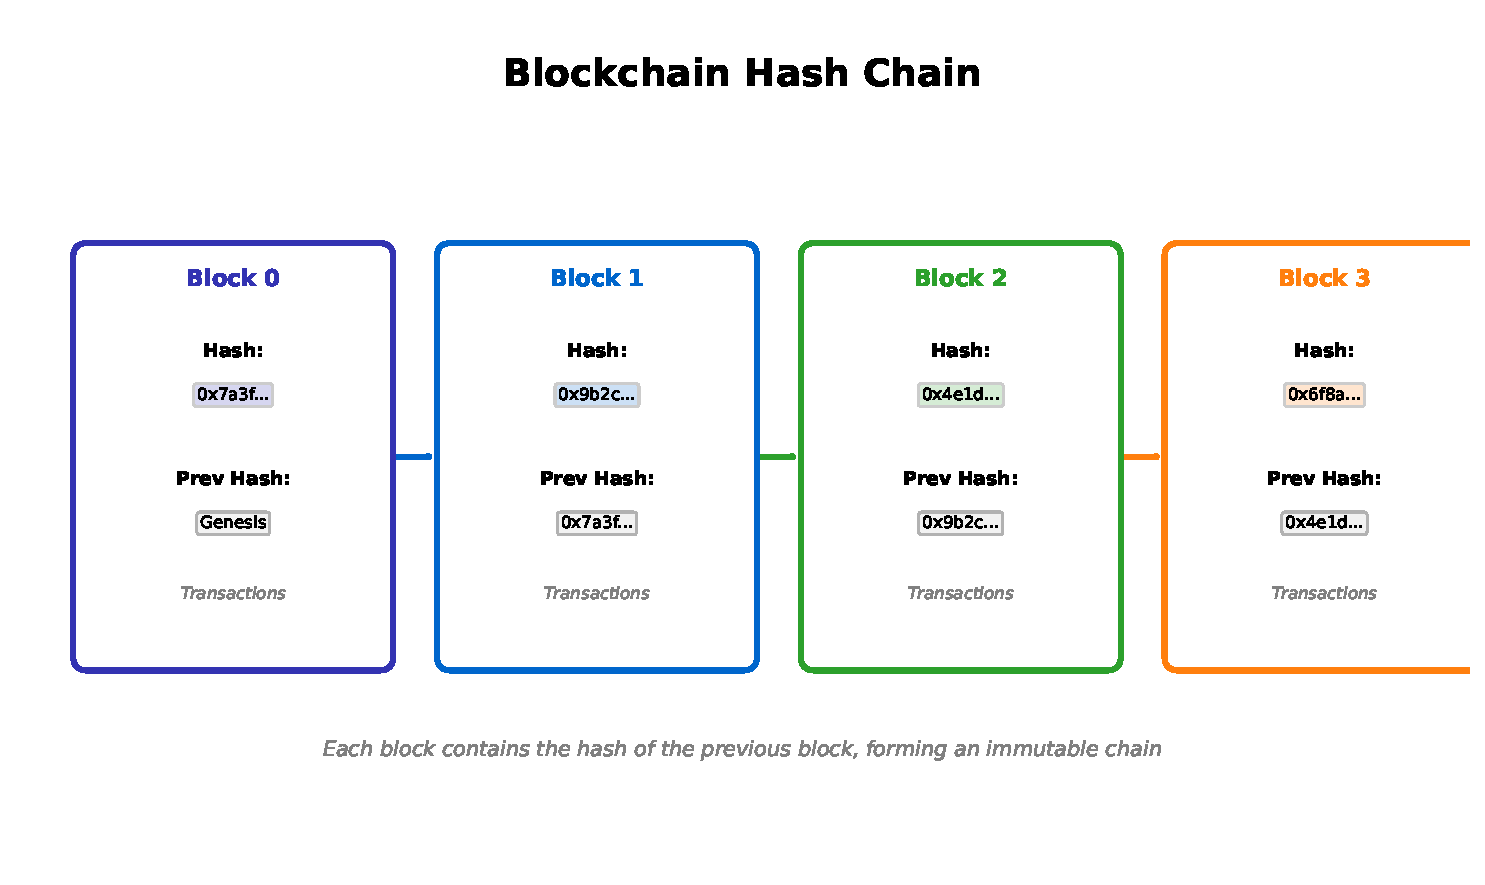
\includegraphics[width=0.95\textwidth]{02_hash_chain/02_hash_chain.pdf}
\end{center}

\vspace{0.3em}
\textbf{The Chain Property:}
\begin{itemize}
\item Each block contains the hash of the previous block
\item This creates a cryptographic chain from genesis to present
\item Modifying any block invalidates all subsequent blocks
\end{itemize}

\bottomnote{This linking mechanism is what makes blockchain ``immutable'' -- tampering is computationally infeasible.}
\end{frame}

% ==================== SLIDE 13: BLOCK CLASS CODE ====================
\begin{frame}[fragile]{Python Implementation: Block Class}
\begin{lstlisting}[style=python]
import hashlib
import time

class Block:
    def __init__(self, index, transactions, previous_hash):
        self.index = index
        self.timestamp = time.time()
        self.transactions = transactions
        self.previous_hash = previous_hash
        self.nonce = 0
        self.hash = self.calculate_hash()

    def calculate_hash(self):
        block_string = f"{self.index}{self.timestamp}{self.transactions}{self.previous_hash}{self.nonce}"
        return hashlib.sha256(block_string.encode()).hexdigest()

    def mine_block(self, difficulty):
        target = "0" * difficulty
        while self.hash[:difficulty] != target:
            self.nonce += 1
            self.hash = self.calculate_hash()
        print(f"Block mined: {self.hash}")
\end{lstlisting}

\bottomnote{This simple implementation captures the core concepts: hashing, linking, and mining.}
\end{frame}

% ==================== SLIDE 14: WHY TAMPERING FAILS ====================
\begin{frame}[t]{Why Tampering Breaks the Chain}
\begin{columns}[T]
\column{0.48\textwidth}
\textbf{Scenario: Attacker modifies Block 2}

\vspace{0.5em}
\begin{enumerate}
\item Attacker changes transaction in Block 2
\item Block 2's hash changes (avalanche effect)
\item Block 3's ``previous hash'' no longer matches
\item Block 3 becomes invalid
\item All subsequent blocks become invalid
\end{enumerate}

\vspace{0.5em}
\textbf{To successfully tamper:}
\begin{itemize}
\item Must recalculate Block 2's hash
\item Must recalculate Block 3's hash
\item Must recalculate ALL subsequent blocks
\item Must outpace the honest network
\end{itemize}

\column{0.48\textwidth}
\textbf{Why this is practically impossible:}

\vspace{0.5em}
\begin{itemize}
\item \textbf{Computational cost:} Each block requires significant work to mine
\item \textbf{Network consensus:} Honest nodes reject invalid chains
\item \textbf{Time factor:} Network continues adding blocks
\item \textbf{51\% attack:} Would need majority hash power
\end{itemize}

\vspace{1em}
\begin{center}
\fbox{\parbox{0.9\columnwidth}{\centering
\textbf{Security guarantee:}\\
Deeper the block, harder to change
}}
\end{center}
\end{columns}

\bottomnote{Bitcoin's security relies on the economic infeasibility of outcomputing the entire network.}
\end{frame}

% ==================== SECTION 3: CONSENSUS ====================
\section{Consensus Mechanisms}

\begin{frame}[t]
\vfill
\centering
\begin{beamercolorbox}[sep=8pt,center]{title}
\usebeamerfont{title}\Large Section 3: Consensus Mechanisms\par
\end{beamercolorbox}
\vfill
\end{frame}

% ==================== SLIDE 15: DOUBLE SPENDING ====================
\begin{frame}[t]{The Double-Spending Problem}
\begin{columns}[T]
\column{0.48\textwidth}
\textbf{The Problem}

\vspace{0.5em}
Digital data can be copied perfectly. How do we prevent someone from spending the same digital money twice?

\vspace{0.5em}
\textbf{Scenario:}
\begin{enumerate}
\item Alice has 10 BTC
\item Alice sends 10 BTC to Bob
\item Alice sends \textit{same} 10 BTC to Charlie
\item Both transactions appear valid!
\end{enumerate}

\vspace{0.5em}
\textbf{Traditional solution:}

Central authority (bank) tracks all balances

\vspace{0.3em}
\textit{But this requires trust...}

\column{0.48\textwidth}
\textbf{Blockchain Solution}

\vspace{0.5em}
\textbf{Consensus mechanism} determines:
\begin{itemize}
\item Which transactions are valid
\item The order of transactions
\item Which version of history is ``true''
\end{itemize}

\vspace{0.5em}
\textbf{Key insight:}

The network agrees on a \textcolor{mlpurple}{\textbf{single, ordered history}}

\vspace{0.5em}
\textbf{Result:}
\begin{itemize}
\item First transaction is accepted
\item Second transaction is rejected
\item No central authority needed
\end{itemize}
\end{columns}

\bottomnote{Solving double-spending without trusted parties was the key innovation of Bitcoin.}
\end{frame}

% ==================== SLIDE 16: PROOF OF WORK ====================
\begin{frame}[t]{Proof of Work (PoW)}
\begin{columns}[T]
\column{0.48\textwidth}
\textbf{The Concept}

\vspace{0.5em}
Miners compete to solve a computational puzzle:

\vspace{0.3em}
\textit{Find a nonce such that:}
$$\text{Hash}(\text{block} + \text{nonce}) < \text{target}$$

\vspace{0.5em}
\textbf{The Process:}
\begin{enumerate}
\item Collect pending transactions
\item Try random nonce values
\item Check if hash meets difficulty
\item First to succeed wins the reward
\item Others verify and accept
\end{enumerate}

\vspace{0.5em}
\textbf{Bitcoin's difficulty:}

Hash must start with $\sim$19 zeros

\column{0.48\textwidth}
\textbf{Why It Works}

\vspace{0.5em}
\textbf{Key properties:}
\begin{itemize}
\item \textbf{Hard to find:} Requires many attempts
\item \textbf{Easy to verify:} One hash check
\item \textbf{Adjustable:} Difficulty adapts
\item \textbf{Fair lottery:} Proportional to hashrate
\end{itemize}

\vspace{0.5em}
\textbf{Economics:}
\begin{itemize}
\item Winner receives block reward
\item Currently 3.125 BTC (post-2024 halving)
\item Plus transaction fees
\end{itemize}

\vspace{0.5em}
\textbf{Cost:} Massive energy consumption
\end{columns}

\bottomnote{PoW makes attacking the network economically irrational -- honest mining is more profitable.}
\end{frame}

% ==================== SLIDE 17: PROOF OF STAKE ====================
\begin{frame}[t]{Proof of Stake (PoS)}
\begin{columns}[T]
\column{0.48\textwidth}
\textbf{The Concept}

\vspace{0.5em}
Validators are chosen based on their ``stake'' (locked cryptocurrency):

\vspace{0.5em}
\textbf{The Process:}
\begin{enumerate}
\item Validators lock up tokens as collateral
\item Algorithm selects validator (weighted random)
\item Selected validator proposes block
\item Other validators attest/verify
\item Valid blocks earn rewards
\end{enumerate}

\vspace{0.5em}
\textbf{Selection factors:}
\begin{itemize}
\item Size of stake
\item Randomization
\item Validator reputation
\end{itemize}

\column{0.48\textwidth}
\textbf{Security Mechanism}

\vspace{0.5em}
\textbf{Slashing:} Bad behavior $\rightarrow$ lose stake

\vspace{0.5em}
\textbf{Punishable actions:}
\begin{itemize}
\item Double-signing (voting twice)
\item Proposing invalid blocks
\item Being offline (mild penalty)
\end{itemize}

\vspace{0.5em}
\textbf{Advantages:}
\begin{itemize}
\item 99.9\%+ less energy
\item No special hardware needed
\item Faster finality possible
\item Economic penalties > physical
\end{itemize}

\vspace{0.5em}
\textbf{Ethereum:} Requires 32 ETH stake
\end{columns}

\bottomnote{PoS achieves security through economic incentives rather than computational work.}
\end{frame}

% ==================== SLIDE 18: POW VS POS ====================
\begin{frame}[t]{Proof of Work vs Proof of Stake}
\begin{center}
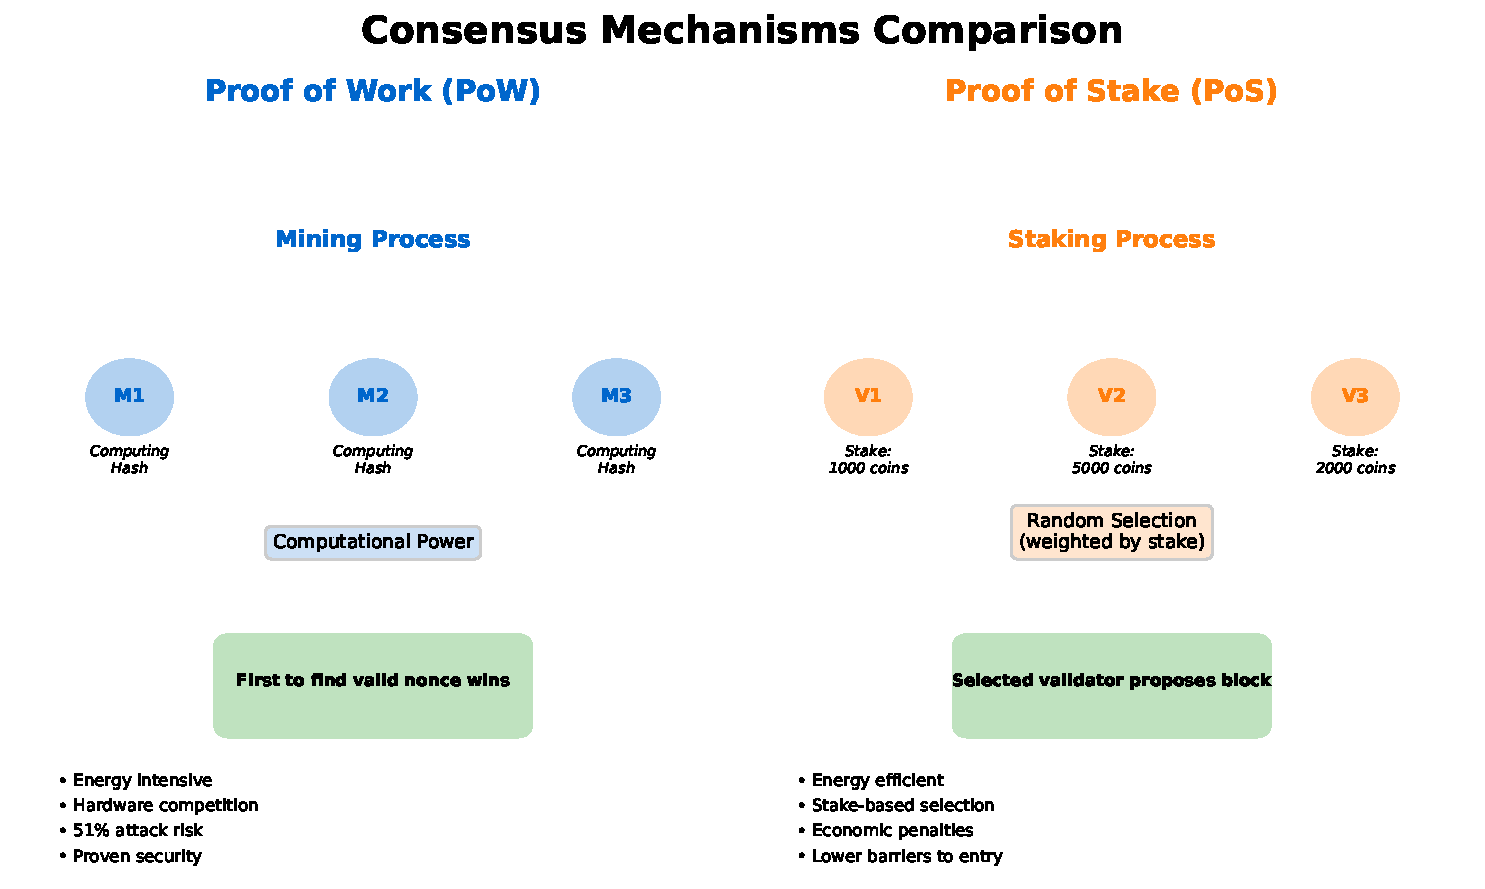
\includegraphics[width=0.95\textwidth]{04_consensus_comparison/04_consensus_comparison.pdf}
\end{center}

\vspace{0.3em}
\begin{center}
\small
\begin{tabular}{lcc}
\toprule
\textbf{Aspect} & \textbf{Proof of Work} & \textbf{Proof of Stake} \\
\midrule
Energy consumption & Very high & Minimal \\
Hardware requirement & Specialized (ASICs) & Standard computer \\
Attack cost & Hardware + electricity & Must own stake \\
Finality & Probabilistic & Can be deterministic \\
Examples & Bitcoin, Litecoin & Ethereum, Cardano, Solana \\
\bottomrule
\end{tabular}
\end{center}

\bottomnote{Both mechanisms aim to solve the same problem: achieving consensus without a central authority.}
\end{frame}

% ==================== SLIDE 19: WHY CONSENSUS MATTERS ====================
\begin{frame}[t]{Why Consensus Matters}
\begin{columns}[T]
\column{0.48\textwidth}
\textbf{Consensus Ensures:}

\vspace{0.5em}
\begin{itemize}
\item[\textcolor{mlgreen}{$\checkmark$}] \textbf{Agreement:} All nodes share same state
\item[\textcolor{mlgreen}{$\checkmark$}] \textbf{Ordering:} Transactions have definitive sequence
\item[\textcolor{mlgreen}{$\checkmark$}] \textbf{Validity:} Only legitimate transactions accepted
\item[\textcolor{mlgreen}{$\checkmark$}] \textbf{Finality:} Confirmed transactions stay confirmed
\item[\textcolor{mlgreen}{$\checkmark$}] \textbf{Liveness:} Network continues making progress
\end{itemize}

\vspace{0.5em}
\textbf{Without consensus:}
\begin{itemize}
\item Different nodes have different ``truths''
\item Double-spending becomes possible
\item Trust in the system collapses
\end{itemize}

\column{0.48\textwidth}
\textbf{The Byzantine Generals Problem}

\vspace{0.5em}
How can distributed parties agree when some may be malicious?

\vspace{0.5em}
\textbf{Requirements:}
\begin{itemize}
\item Majority must be honest
\item Communication may be unreliable
\item Some generals (nodes) may lie
\end{itemize}

\vspace{0.5em}
\textbf{Blockchain's solution:}

Economic incentives align behavior:
\begin{itemize}
\item Honest participation is profitable
\item Attacks are expensive
\item Security from game theory
\end{itemize}
\end{columns}

\bottomnote{Consensus is what transforms a distributed database into a trustworthy source of truth.}
\end{frame}

% ==================== SECTION 4: PYTHON DEMO ====================
\section{Python Implementation}

\begin{frame}[t]
\vfill
\centering
\begin{beamercolorbox}[sep=8pt,center]{title}
\usebeamerfont{title}\Large Section 4: Python Implementation\par
\end{beamercolorbox}
\vfill
\end{frame}

% ==================== SLIDE 20: ARCHITECTURE ====================
\begin{frame}[t]{Our Simple Blockchain Architecture}
\begin{columns}[T]
\column{0.48\textwidth}
\textbf{Components}

\vspace{0.5em}
\textbf{1. Block Class}
\begin{itemize}
\item Index (position in chain)
\item Timestamp
\item Transaction data
\item Previous hash
\item Nonce (for mining)
\item Hash (calculated)
\end{itemize}

\vspace{0.5em}
\textbf{2. Blockchain Class}
\begin{itemize}
\item Chain (list of blocks)
\item Difficulty setting
\item Genesis block creation
\item Block addition
\item Chain validation
\end{itemize}

\column{0.48\textwidth}
\textbf{Simplifications}

\vspace{0.5em}
Our demo omits (for clarity):
\begin{itemize}
\item Network communication
\item Transaction signatures
\item UTXO model
\item Merkle trees
\item Difficulty adjustment
\end{itemize}

\vspace{0.5em}
\textbf{Core concepts preserved:}
\begin{itemize}
\item[\textcolor{mlgreen}{$\checkmark$}] Cryptographic hashing
\item[\textcolor{mlgreen}{$\checkmark$}] Block linking
\item[\textcolor{mlgreen}{$\checkmark$}] Proof of Work mining
\item[\textcolor{mlgreen}{$\checkmark$}] Chain validation
\item[\textcolor{mlgreen}{$\checkmark$}] Tamper detection
\end{itemize}
\end{columns}

\bottomnote{This implementation captures the essential mechanics while remaining understandable.}
\end{frame}

% ==================== SLIDE 21: BLOCK CLASS ====================
\begin{frame}[fragile]{Code: Block Class}
\begin{lstlisting}[style=python]
import hashlib
import time

class Block:
    def __init__(self, index, transactions, previous_hash):
        self.index = index                    # Position in chain
        self.timestamp = time.time()          # Creation time
        self.transactions = transactions      # Data payload
        self.previous_hash = previous_hash    # Link to parent
        self.nonce = 0                        # Mining counter
        self.hash = self.calculate_hash()     # Block's fingerprint

    def calculate_hash(self):
        """Combine all fields and hash them."""
        block_string = f"{self.index}{self.timestamp}{self.transactions}"
        block_string += f"{self.previous_hash}{self.nonce}"
        return hashlib.sha256(block_string.encode()).hexdigest()

    def mine_block(self, difficulty):
        """Find a nonce that produces a hash with required leading zeros."""
        target = "0" * difficulty
        while self.hash[:difficulty] != target:
            self.nonce += 1
            self.hash = self.calculate_hash()
        print(f"Block {self.index} mined: {self.hash}")
\end{lstlisting}

\bottomnote{The \texttt{mine\_block} method implements Proof of Work -- finding a valid nonce.}
\end{frame}

% ==================== SLIDE 22: BLOCKCHAIN CLASS ====================
\begin{frame}[fragile]{Code: Blockchain Class}
\begin{lstlisting}[style=python]
class Blockchain:
    def __init__(self, difficulty=2):
        self.chain = [self.create_genesis_block()]  # Start with genesis
        self.difficulty = difficulty                 # Mining difficulty

    def create_genesis_block(self):
        """Create the first block in the chain."""
        return Block(0, "Genesis Block", "0")

    def get_latest_block(self):
        """Return the most recent block."""
        return self.chain[-1]

    def add_block(self, transactions):
        """Create and mine a new block, then add to chain."""
        new_block = Block(
            len(self.chain),                    # Next index
            transactions,                        # Transaction data
            self.get_latest_block().hash        # Link to previous
        )
        new_block.mine_block(self.difficulty)   # Do the work
        self.chain.append(new_block)            # Add to chain
\end{lstlisting}

\bottomnote{Each new block references the previous block's hash, creating the chain.}
\end{frame}

% ==================== SLIDE 23: MINING DEMO ====================
\begin{frame}[fragile]{Code: Mining Demonstration}
\begin{lstlisting}[style=python]
if __name__ == "__main__":
    # Create blockchain with difficulty 2 (hash must start with "00")
    print("Creating blockchain with difficulty 2...")
    bc = Blockchain(difficulty=2)

    # Add some transactions
    print("\nAdding transactions...")
    bc.add_block("Alice sends 10 BTC to Bob")
    bc.add_block("Bob sends 5 BTC to Charlie")
    bc.add_block("Charlie sends 2 BTC to Dave")
\end{lstlisting}

\vspace{0.5em}
\textbf{Expected Output:}
\begin{lstlisting}[style=python,numbers=none]
Creating blockchain with difficulty 2...

Adding transactions...
Block 1 mined: 00a7f3b2c4d5e6f7...  (found after ~256 attempts)
Block 2 mined: 003e8f9a1b2c3d4e...  (found after ~512 attempts)
Block 3 mined: 00d4c5b6a7980123...  (found after ~128 attempts)
\end{lstlisting}

\bottomnote{Higher difficulty = more leading zeros required = exponentially more attempts needed.}
\end{frame}

% ==================== SLIDE 24: VALIDATION CODE ====================
\begin{frame}[fragile]{Code: Chain Validation}
\begin{lstlisting}[style=python]
def is_chain_valid(self):
    """Verify the integrity of the entire blockchain."""
    for i in range(1, len(self.chain)):
        current = self.chain[i]
        previous = self.chain[i-1]

        # Check 1: Hash must be valid
        if current.hash != current.calculate_hash():
            print(f"Block {i}: Hash mismatch!")
            return False

        # Check 2: Previous hash must match
        if current.previous_hash != previous.hash:
            print(f"Block {i}: Chain broken!")
            return False

    return True

# Test validation
print(f"\nBlockchain valid: {bc.is_chain_valid()}")  # True

# Attempt tampering
bc.chain[1].transactions = "Alice sends 1000 BTC to Eve"
print(f"After tampering: {bc.is_chain_valid()}")    # False
\end{lstlisting}

\bottomnote{Tampering changes the hash, which breaks the chain link -- instantly detectable.}
\end{frame}

% ==================== SLIDE 25: LIVE DEMO ====================
\begin{frame}[t]{Live Demo: Try It Yourself}
\begin{columns}[T]
\column{0.48\textwidth}
\textbf{Running the Demo}

\vspace{0.5em}
\begin{enumerate}
\item Navigate to the code directory:
\begin{center}
\texttt{cd code/}
\end{center}

\item Run the complete demo:
\begin{center}
\texttt{python simple\_blockchain.py}
\end{center}

\item Observe:
\begin{itemize}
\item Block mining output
\item Hash values
\item Validation results
\item Tampering detection
\end{itemize}
\end{enumerate}

\column{0.48\textwidth}
\textbf{Experiments to Try}

\vspace{0.5em}
\textbf{1. Change difficulty:}
\begin{itemize}
\item Set \texttt{difficulty=3}
\item Notice mining takes longer
\item Each +1 difficulty $\approx$ 16x slower
\end{itemize}

\vspace{0.5em}
\textbf{2. Tamper with blocks:}
\begin{itemize}
\item Modify a transaction
\item Run validation
\item See it fail
\end{itemize}

\vspace{0.5em}
\textbf{3. Add more blocks:}
\begin{itemize}
\item Create longer chain
\item Validate entire chain
\end{itemize}
\end{columns}

\bottomnote{Hands-on experimentation is the best way to understand blockchain mechanics.}
\end{frame}

% ==================== SECTION 5: SUMMARY ====================
\section{Summary}

\begin{frame}[t]
\vfill
\centering
\begin{beamercolorbox}[sep=8pt,center]{title}
\usebeamerfont{title}\Large Section 5: Summary\par
\end{beamercolorbox}
\vfill
\end{frame}

% ==================== SLIDE 26: KEY TAKEAWAYS ====================
\begin{frame}[t]{Key Takeaways}
\begin{columns}[T]
\column{0.48\textwidth}
\textbf{Blockchain Fundamentals}
\begin{enumerate}
\item \textbf{Distributed ledger:} No central authority
\item \textbf{Immutability:} Cryptographic linking prevents tampering
\item \textbf{Consensus:} Network agrees on truth
\item \textbf{Transparency:} Anyone can verify
\end{enumerate}

\vspace{0.5em}
\textbf{Block Structure}
\begin{itemize}
\item Header: metadata (hash, prev\_hash, nonce)
\item Body: transaction data
\item Merkle root: efficient verification
\end{itemize}

\column{0.48\textwidth}
\textbf{Consensus Mechanisms}
\begin{itemize}
\item \textbf{PoW:} Computational work proves legitimacy
\item \textbf{PoS:} Economic stake proves commitment
\item Both solve double-spending
\end{itemize}

\vspace{0.5em}
\textbf{Core Innovation}

\vspace{0.3em}
\begin{center}
\fbox{\parbox{0.9\columnwidth}{\centering
\textit{``Don't trust, verify''}\\[0.3em]
Blockchain enables trustless transactions between strangers through cryptography and game theory
}}
\end{center}
\end{columns}

\bottomnote{These fundamentals apply to all blockchains -- Bitcoin, Ethereum, and beyond.}
\end{frame}

% ==================== SLIDE 27: CENTRALIZED VS DECENTRALIZED ====================
\begin{frame}[t]{Centralized vs Decentralized Networks}
\begin{center}
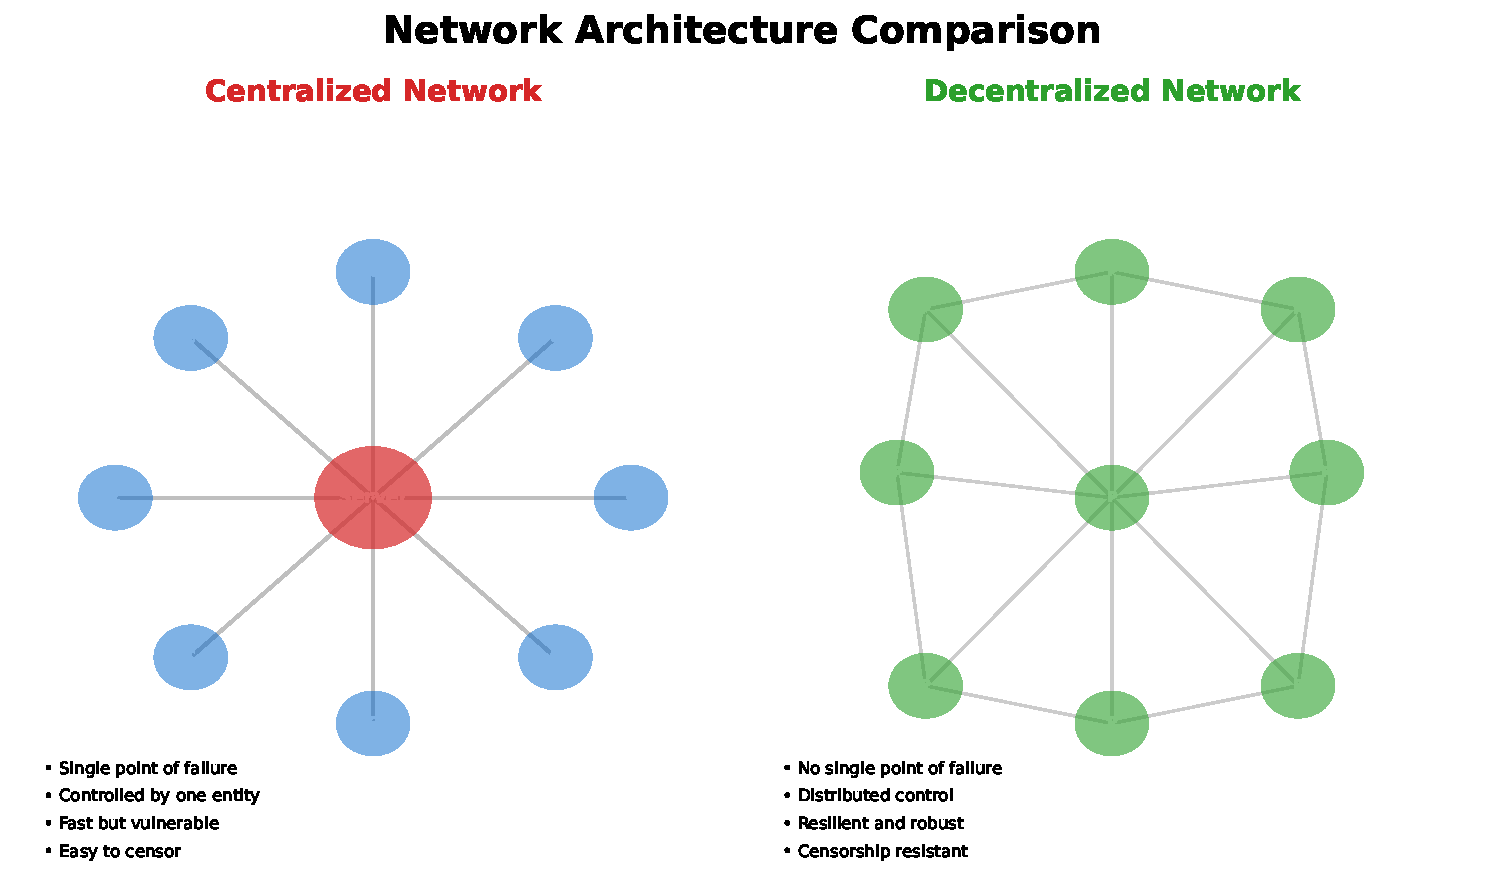
\includegraphics[width=0.95\textwidth]{05_decentralization/05_decentralization.pdf}
\end{center}

\vspace{0.3em}
\begin{center}
\textbf{Key difference:} Decentralization trades efficiency for resilience, censorship resistance, and trustlessness.
\end{center}

\bottomnote{Most real systems exist on a spectrum between fully centralized and fully decentralized.}
\end{frame}

% ==================== SLIDE 28: NEXT LESSON ====================
\begin{frame}[t]{Coming Up: Lesson 2 -- Cryptography}
\begin{columns}[T]
\column{0.48\textwidth}
\textbf{Topics We'll Cover}

\vspace{0.5em}
\begin{itemize}
\item Hash functions in depth
\begin{itemize}
\item SHA-256 internals
\item Properties and security
\end{itemize}
\item Public key cryptography
\begin{itemize}
\item Key pairs
\item Elliptic curves
\end{itemize}
\item Digital signatures
\begin{itemize}
\item ECDSA
\item Transaction signing
\end{itemize}
\item Addresses and wallets
\end{itemize}

\column{0.48\textwidth}
\textbf{Why Cryptography Matters}

\vspace{0.5em}
Cryptography provides:
\begin{itemize}
\item[\textcolor{mlblue}{$\rightarrow$}] \textbf{Integrity:} Data hasn't been changed
\item[\textcolor{mlgreen}{$\rightarrow$}] \textbf{Authentication:} Proves identity
\item[\textcolor{mlorange}{$\rightarrow$}] \textbf{Non-repudiation:} Can't deny signing
\item[\textcolor{mlpurple}{$\rightarrow$}] \textbf{Privacy:} Selective disclosure
\end{itemize}

\vspace{1em}
\textbf{Preparation:}
\begin{itemize}
\item Review modular arithmetic
\item Basic understanding of prime numbers
\end{itemize}
\end{columns}

\bottomnote{Cryptography is the foundation that makes blockchain security possible.}
\end{frame}

% ==================== SLIDE 29: QUESTIONS ====================
\begin{frame}[plain]
\vspace{3cm}
\begin{center}
{\Large Questions?}\\[2cm]
{\normalsize Discussion Topics:}\\[0.5cm]
\begin{itemize}
\centering
\item[] What problems could blockchain solve in your field?
\item[] When is a blockchain \textit{not} the right solution?
\item[] How might PoW and PoS evolve?
\end{itemize}
\end{center}
\end{frame}

% ==================== SLIDE 30: RESOURCES ====================
\begin{frame}[t]{Resources and References}
\begin{columns}[T]
\column{0.48\textwidth}
\textbf{Essential Reading}
\begin{itemize}
\item Nakamoto, S. (2008): \textit{Bitcoin: A Peer-to-Peer Electronic Cash System}
\item Antonopoulos, A.: \textit{Mastering Bitcoin} (O'Reilly)
\item Narayanan et al.: \textit{Bitcoin and Cryptocurrency Technologies}
\end{itemize}

\vspace{0.5em}
\textbf{Online Resources}
\begin{itemize}
\item bitcoin.org -- Official documentation
\item ethereum.org -- Ethereum docs
\item blockchain.com -- Block explorer
\end{itemize}

\column{0.48\textwidth}
\textbf{Interactive Learning}
\begin{itemize}
\item Anders Brownworth's blockchain demo
\item CryptoZombies (Solidity)
\item Coursera: Bitcoin and Cryptocurrencies
\end{itemize}

\vspace{0.5em}
\textbf{Course Materials}
\begin{itemize}
\item Slides and code available online
\item Python examples: \texttt{code/} directory
\item Practice exercises in assignments
\end{itemize}

\vspace{0.5em}
\textbf{Contact:}\\
\small joerg.osterrieder@uni.edu
\end{columns}

\bottomnote{The Bitcoin whitepaper is only 9 pages -- highly recommended reading!}
\end{frame}

\end{document}
